%%%%%%%%%%%%%%%%%%%%%%%%%%%%%%%%%%%%%%%%%%%%%%%%%%%%%%%%%%%%%%%%%%%%%%%%%%%%%%%%%%%%%%
% Modelo de relatório de Disciplina de MLP a partir da
% classe latex iiufrgs disponivel em http://github.com/schnorr/iiufrgs
%%%%%%%%%%%%%%%%%%%%%%%%%%%%%%%%%%%%%%%%%%%%%%%%%%%%%%%%%%%%%%%%%%%%%%%%%%%%%%%%%%%%%%

%%%%%%%%%%%%%%%%%%%%%%%%%%%%%%%%%%%%%%%%%%%%%%%%%%%%%%%%%%%%%%%%%%%%%%%%%%%%%%%%%%%%%%
% Definição do tipo / classe de documento e estilo usado
%%%%%%%%%%%%%%%%%%%%%%%%%%%%%%%%%%%%%%%%%%%%%%%%%%%%%%%%%%%%%%%%%%%%%%%%%%%%%%%%%%%%%%
%
\documentclass[rel_mlp]{iiufrgs}

%%%%%%%%%%%%%%%%%%%%%%%%%%%%%%%%%%%%%%%%%%%%%%%%%%%%%%%%%%%%%%%%%%%%%%%%%%%%%%%%%%%%%%
% Importação de pacotes
%%%%%%%%%%%%%%%%%%%%%%%%%%%%%%%%%%%%%%%%%%%%%%%%%%%%%%%%%%%%%%%%%%%%%%%%%%%%%%%%%%%%%%
% (a A seguir podem ser importados os pacotes necessários para o documento, de acordo 
% com a necessidade)
%
\usepackage[brazilian]{babel}	    % para texto escrito em pt-br
\usepackage[utf8]{inputenc}         % pacote para acentuação
\usepackage{graphicx}         	    % pacote para importar figuras
\usepackage[T1]{fontenc}            % pacote para conj. de caracteres correto
\usepackage{times}                  % pacote para usar fonte Adobe Times
\usepackage{enumerate}              % para lista de itens com letras
\usepackage{breakcites}
\usepackage{titlesec}
\usepackage{enumitem}
\usepackage{titletoc}               
\usepackage{listings}			    % para listagens de código-fonte
\usepackage{mathptmx}               % p/ usar fonte Adobe Times nas formulas matematicas
\usepackage{url}                    % para formatar URLs
%\usepackage{color}				    % para imagens e outras coisas coloridas
%\usepackage{fixltx2e}              % para subscript
\usepackage{amsmath}               % para \epsilon e matemática
%\usepackage{amsfonts}
%\usepackage{setspace}			    % para mudar espaçamento dos parágrafos
%\usepackage[table,xcdraw]{xcolor}  % para tabelas coloridas
%\usepackage{longtable}             % para tabelas compridas (mais de uma página)
%\usepackage{float}
%\usepackage{booktabs}
%\usepackage{tabularx}
%\usepackage[breaklinks]{hyperref}
\usepackage{pdfpages}

\usepackage[alf,abnt-emphasize=bf]{abntex2cite}	% pacote para usar citações abnt

\graphicspath{ {images/} }

%%%%%%%%%%%%%%%%%%%%%%%%%%%%%%%%%%%%%%%%%%%%%%%%%%%%%%%%%%%%%%%%%%%%%%%%%%%%%%%%%%%%%%
% Macros, ajustes e definições
%%%%%%%%%%%%%%%%%%%%%%%%%%%%%%%%%%%%%%%%%%%%%%%%%%%%%%%%%%%%%%%%%%%%%%%%%%%%%%%%%%%%%%
%

% define estilo de parágrafo para citação longa direta:
\newenvironment{citacao}{
    %\singlespacing
    %\footnotesize
    \small
    \begin{list}{}{
        \setlength{\leftmargin}{4.0cm}
        \setstretch{1}
        \setlength{\topsep}{1.2cm}
        \setlength{\listparindent}{\parindent}
    }
    \item[]}{\end{list}
}

% adiciona a fonte em figuras e tabelas
\newcommand{\fonte}[1]{\\Fonte: {#1}}

% Ative o seguinte caso alguma nota de rodapé fique muito longa e quebre entre múltiplas
% páginas
%\interfootnotelinepenalty=10000

\numberwithin{figure}{chapter}

%%%%%%%%%%%%%%%%%%%%%%%%%%%%%%%%%%%%%%%%%%%%%%%%%%%%%%%%%%%%%%%%%%%%%%%%%%%%%%%%%%%%%%
% Informações gerais                                   
%%%%%%%%%%%%%%%%%%%%%%%%%%%%%%%%%%%%%%%%%%%%%%%%%%%%%%%%%%%%%%%%%%%%%%%%%%%%%%%%%%%%%%

% título
\title{Implementação do jogo de tabuleiro War em Typescript usando os paradigmas funcional e orientado a objetos}

% autor
\author{Moraes}{Alex} % {sobrenome}{nome}
\author{Santana}{Bruno}
\author{Weit}{João} % {sobrenome}{nome} 1 para cada aluno

% Professor orientador da disciplina
\advisor[Prof.~Dr.]{Mello Schnorr}{Lucas}

% Nome do(s) curso(s):
\course{Curso de Graduação em Ciência da Computa{\c{c}}{\~a}o e Engenharia de Computação}

% local da realização do trabalho 
\location{Porto Alegre}{RS} 

% data da entrega do trabalho (mês e ano)
\date{07}{2018}


% Palavras chave
\keyword{Typescript}
\keyword{Functional}
\keyword{Object oriented}


%%%%%%%%%%%%%%%%%%%%%%%%%%%%%%%%%%%%%%%%%%%%%%%%%%%%%%%%%%%%%%%%%%%%%%%%%%%%%%%%%%%%%%
% Início do documento e elementos pré-textuais
%%%%%%%%%%%%%%%%%%%%%%%%%%%%%%%%%%%%%%%%%%%%%%%%%%%%%%%%%%%%%%%%%%%%%%%%%%%%%%%%%%%%%%

% Declara início do documento
\begin{document}

% inclui folha de rosto 
\maketitle      

\selectlanguage{brazilian}



% Sumario
\tableofcontents



%%%%%%%%%%%%%%%%%%%%%%%%%%%%%%%%%%%%%%%%%%%%%%%%%%%%%%%%%%%%%%%%%%%%%%%%%%%%%%%%%%%%%
% Aqui comeca o texto propriamente dito
%%%%%%%%%%%%%%%%%%%%%%%%%%%%%%%%%%%%%%%%%%%%%%%%%%%%%%%%%%%%%%%%%%%%%%%%%%%%%%%%%%%%%

%espaçamento entre parágrafos
%\setlength{\parskip}{6 pt}

\selectlanguage{brazilian}



%%%%%%%%%%%%%%%%%%%%%%%%%%%%%%%%%%%%%%%%%%%%%%%%%%%%%%%%%%%%%%%%%%%%%%%%%%%%%%%%%%%%%
% Introdução
%
\chapter{Introdução} \label{intro}

Este trabalho tem por objetivo a implementação de uma aplicação em uma linguagem que suporte tanto o paradigma funcional quanto o paradigma orientado a objetos visando a comparação das duas abordagens na solução de um mesmo problema. A aplicação escolhida pelo grupo é uma versão eletrônica do jogo de tabuleiro \textit{War} que será desenvolvida usando a linguagem TypeScript.

\section{TypeScript}

TypeScript é um superconjunto da linguagem JavaScript desenvolvida pela Microsoft, projetada com o objetivo de reduzir a complexidade de código produzido em JavaScript. Ao contrário de JavaScript, TypeScript é uma linguagem compilada e o produto final da compilação é código em JavaScript que pode ser interpertado por qualquer motor que suporte o padrão ECMAScript 3 ou superior.

Outra diferença em relação a sua predecessora é a possibilidade de tipagem estática. Quando são adicionadas anotações de tipo às declarações, a checagem de tipos é feita em tempo de compilação. Adicionalmente, existe a possibilidade do uso de classes, interfaces, módulos e \textit{namespaces}. Além disso, sendo uma extensão do padrão ECMAScript 5, qualquer programa em JavaScript é um programa TypeScript válido.


\section{Paradigma funcional}

O paradigma funcional é uma maneira distinta da qual estamos acostumados de se descrever uma determinada computação. Diferente do paradigma imperativo, em funcional tudo é representado por funções matemáticas, sem estados ou efeitos colaterais, isto é, toda vez que uma função for executada, deve retornar o mesmo valor e não deve alterar nada externo à ela. Além disso, por ser um paradigma \textit{declarativo}, a ordem de execução do programa não pode ser definida, tornando o mesmo altamente paralelizável.

\section{Paradigma orientado a objetos}

O paradigma orientado a objetos visa um forte mapeamento entre objetos do mundo real e objetos do programa, geralmente representados por classes. A orientação a objetos possui como base os conceitos de abstração de dados, encapsulamento, herança e polimorfismo, tornando o código gerado muito mais legível e de fácil reuso. Todas essas características têm como objetivo aproximar o software desenvolvido do mundo real, tornando o sistema extremamente modular e de fácil interpretação quando feito corretamente.


\chapter{Visão geral da linguagem}

A linguagem definida para o desenvolvimento do trabalho foi Typescript, uma linguagem de código aberto desenvolvida pela Microsoft, que propõe orientação a objetos e compila em Javascript nativo. Por Javascript ser altamente portável - todos navegadores são capazes de executar javascript - Typescript acabou se tornando uma ótima opção para orientação a objetos em aplicações que necessitam rodar em navegadores. A principal adição do Typescript em relação ao Javascript notoriamente é a noção de orientação a objetos, permitindo a criação de classes, tipos estáticos, interfaces, entre outros - mais detalhes sobre estas e outras funcionalidades de orientação a objetos serão abordadas durante este trabalho. Typescript veio para substituir o Javascript nativo em projetos grandes, tornando as suas manutenções uma tarefa fácil, devido às grandes e já conhecidas vantagens de manutenção em códigos orientados a objetos, que são: abstração, encapsulamento, herança e polimorfismo. Mesmo Typescript sendo uma linguagem relativamente nova - lançado em fevereiro de 2017 -, o seu uso em aplicações comercias vem crescendo consideravelmente, graças à compatibilidade com Javascript, o que propõe migrações parciais de código para a nova linguagem. Uma das aplicações que possui implementações em Typescript é o VSCode, que é uma IDE altamente usada na indústria e foi inclusive a IDE escolhida para realizarmos a implementação deste trabalho.

\chapter{Apresentação do problema}

\begin{figure}
\centering {
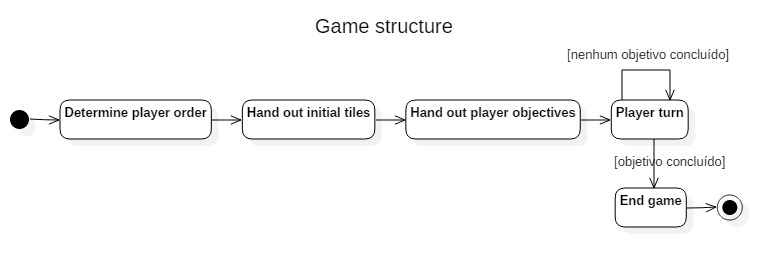
\includegraphics[width=130mm, scale=0.6]{images/Model__Game__Game_1.jpg}
}
\caption{Representação em máquina de estados das etapas do jogo}
\legend{Fonte: Os Autores}
\label{fig:smGame}
\end{figure}

\begin{figure}
\centering {
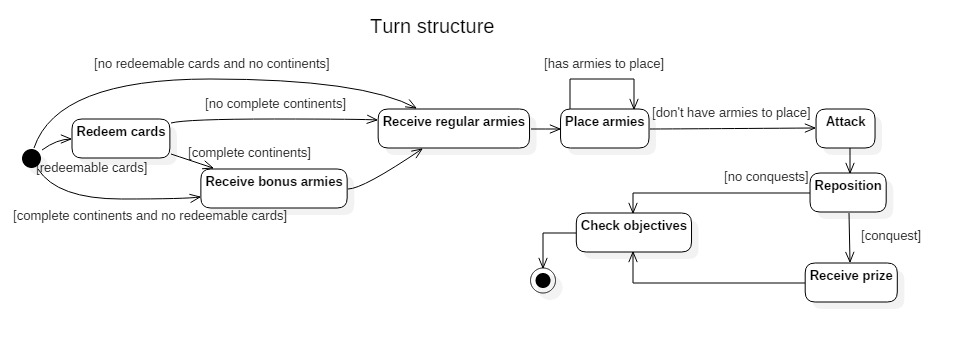
\includegraphics[width=130mm, scale=0.6]{images/Model__Turn__Turn_2.jpg}
}
\caption{Representação em máquina de estados das etapas do turno}
\legend{Fonte: Os Autores}
\label{fig:smTurn}
\end{figure}

O jogo de tabuleiro \textit{War} (\textit{Risk} na sua versão orignal) é um jogo de estratégia no qual cada jogador controla exércitos em uma missão de dominação mundial. A dinâmica do jogo consiste em expandir o seu domínio sobre o tabuleiro participando de combates contra os exércitos dos outros jogadores \cite{riskMan}.

Na etapa inicial do jogo, cada jogador escolhe para si, em turnos, um território desocupado do tabuleiro até que não existam mais territórios desocupados. Em cada um dos territórios escolhidos, o jogador coloca uma peça representando o seu exército de ocupaçao no território. Em seguida cada jogador recebe uma quantidade de exércitos definida de acordo com a quantidade de jogadores. Os jogadores também se revezam em turnos posicionando cada um desses exércitos em territórios sob o seu controle. Quando todos os exércitos são posicionados dessa forma, o jogo avança para a próxima etapa.

Na etapa seguinte, os jogadores ser revezam em turnos onde reforçam as suas posições em territórios já ocupados e combatem os exércitos dos territórios dos oponentes. Cada turno começa com o jogador ativo recebendo exércitos de acordo com a quantidade de territórios possuídos e os posicionando em seus territórios. Uma vez que todos os exércitos do turno tenham sido posicionados, o jogador pode escolher qualquer território seu que possui mais de um exército e declarar um ataque contra um território vizinho que seja controlado por um oponente. Em cada turno, o jogador pode escolher atacar quantas vezes quiser desde que possua territórios com mais de um exército.

No combate, o jogador atacante escolhe até 3 exércitos no território atacante e rola um dado de ataque para cada exército escolhido. O jogador defensor escolhe até 2 exércitos no território atacado e rola um dado de defesa para cada exército escolhido. A maior rolagem de ataque é então comparada com a maior rolagem de defesa e, caso seja maior, um exército do território atacado é removido do tabuleiro. Caso a rolagem de ataque seja igual ou menor que a rolagem de defesa, um exército do território atacante é removido. Esse procedimento se repete para as próximas maiores rolagens de ataque e defesa enquanto houverem dados para serem comparados. Ao final desse processo, se o território atacado acabar sem exércitos, o jogador atacante move os exércitos atacantes que restaram para esse território.

O sequênciamento dessas ações no jogo podem ser representadas por máquinas de estados e essa representação foi a que guiou o desenvolvimento da solução. A Figura \ref{fig:smGame} representa a sequência de etapas do jogo, a Figura \ref{fig:smTurn} representa a sequências de fases de um turno e a Figura \ref{fig:smAttack} representa as etapas de um combate.

\begin{figure}
\centering {
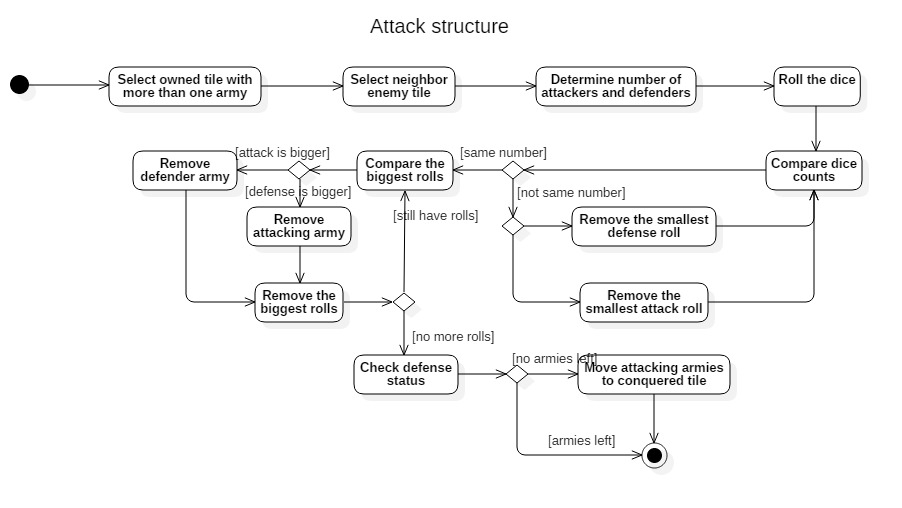
\includegraphics[width=130mm, scale=0.6]{images/Model__Attack__Attack_4.jpg}
}
\caption{Representação em máquina de estados das etapas do combate}
\legend{Fonte: Os Autores}
\label{fig:smAttack}
\end{figure}





%%%%%%%%%%%%%%%%%%%%%%%%%%%%%%%%%%%%%%%%%%%%%%%%%%%%%%%%%%%%%%%%%%%%%%%%%%%%%%%%%%%%%
% Capítulo 3
%
\chapter{Abordagem orientada a objetos}

\section{Classes}

As classes são a base da orientação a objetos. A figura 4.1 representa o diagrama de classes UML modelado para este projeto e utilizado como base para implementação do mesmo.
\begin{figure}[ht]
\centering {
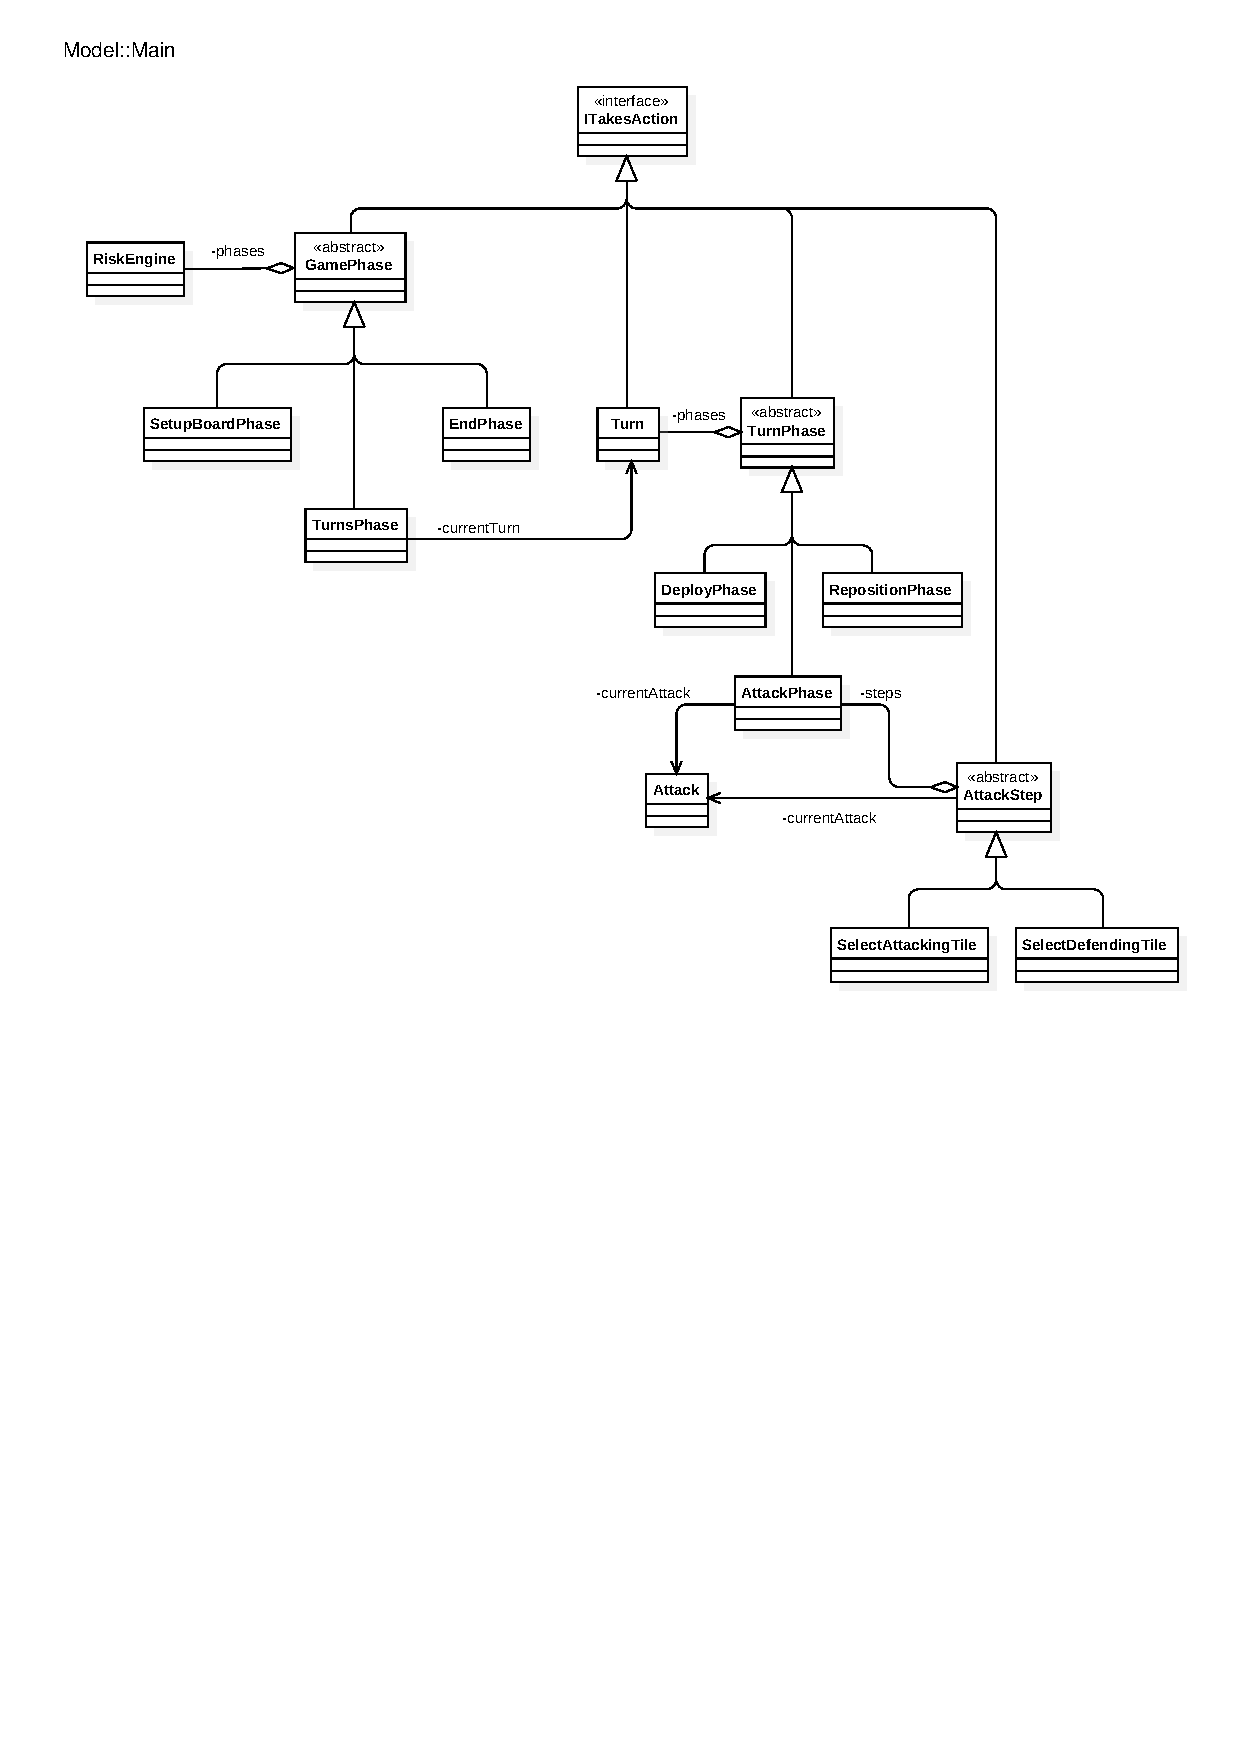
\includegraphics[width=130mm, scale=0.6]{uml/ClassDiagram.pdf}
}
%\lstinputlisting[firstline=37, lastline=45]{../src/classes/RiskEngine.ts}
%\lstinputlisting{../src/Interfaces/IRisk.ts}
\caption{Typescript class}
\label{fig:tsClass}
\end{figure}


\section{Encapsulamento}

O encapsulamento envolve a abstração dos métodos e atributos de determinada classe, tornando o software mais flexível à mudanças, já que cada funcionalidade deve ser implementada isolada das demais. Quando se usa orientação a objetos, o encapsulamento é muito mais simples de ser atingido, pois o código é organizado em classes.

\section{Construtores}

Os construtores são métodos chamados ao instanciar um objeto, podendo ser herdados de uma classe abstrata à qual a classe em questão herda ou ser definidos na própria classe. Como o conceito de herança foi amplamente utilizado neste projeto, grande parte dos objetos herda o construtor de sua superclasse, mas em alguns casos extendemos o construtor herdado para atingir alguma funcionalidade a mais implementada pela classe filha, como pode ser observado na classe \textit{SetupBoardPhase}, mostrado na Figura 4.2.

\begin{figure}[ht]
\centering {
	\lstinputlisting[firstline=4, lastline=8]{../src/classes/gamePhases/SetupBoardPhase.ts}
}
%\lstinputlisting[firstline=37, lastline=45]{../src/classes/RiskEngine.ts}
%\lstinputlisting{../src/Interfaces/IRisk.ts}
\caption{Construtor da classe \textit{SetupBoardPhase}}
\label{fig:tsClass}
\end{figure}

 
\section{Destrutores}

Em typescript temos o conceito de \textit{garbage collection}, um processo automático que desaloca objetos que não são mais referenciados no programa. Com esta tecnologia, o programador não precisa se preocupar com o gerenciamento de memória e evita problemas como o \textit{memory leak}. Tendo este recurso disponível, destrutores se tornam desnecessários na linguagem. Porém, esta funcionalidade da linguagem também possui desvantagens, tal como o maior uso de recursos computacionais para definir que objetos podem ser desalocados, visto que em linguagens que não possuem garbage collection, o programador que gerencia a desalocação de memória, resultando em menor uso destes recursos.
\cite{memMng}


%\section{Namespaces}

%\section{Herança}

\section{Polimorfismo por inclusão}

O polimorfismo por inclusão é aquele em que um objeto pode pertencer a várias classes, tendo um comportamento modificado em relação ao comportamento original. 
Neste trecho de código, o polimorfismo por inclusão ocorre pois a propriedade \textit{this.phases} é um Array de \textit{TurnPhase} e este Array foi inicializado no construtor com dois elementos, o primeiro sendo o DeployPhase e o segundo o AttackPhase. Estas são classes que modificam comportamentos da classe \textit{TurnPhase} e serão tratados como \textit{TurnPhase} a partir de então. Posteriormente, por exemplo, o método \textit{takeAction()} será chamado para cada elemento do Array de \textit{TurnPhase}, sendo executado a implementação da classe herdada - \textit{DeployPhase} ou \textit{AttackPhase}.

\begin{figure}[ht]
\centering {
	\lstinputlisting[firstline=8, lastline=11]{../src/classes/Turn.ts}
}
%\lstinputlisting[firstline=37, lastline=45]{../src/classes/RiskEngine.ts}
%\lstinputlisting{../src/Interfaces/IRisk.ts}
\caption{Trecho do construtor da classe \textit{Turn}}
\label{fig:tsClass}
\end{figure}

\section{Polimorfismo por sobrecarga}

O polimorfismo por sobrecarga acontece quando usamos um mesmo método com parâmetros diferentes. Não usamos no trabalho pois TypeScript não suporta sobrecarga de operandos.


%%%%%%%%%%%%%%%%%%%%%%%%%%%%%%%%%%%%%%%%%%%%%%%%%%%%%%%%%%%%%%%%%%%%%%%%%%%%%%%%%%%%%
% Capítulo 5
%
\chapter{Abordagem funcional}

\section{Funções Lambda}

Funções lambda, ou funções anonimas, são funções que essencialmente não possuem nome ou identificador, e geralmente são armazenadas em variáveis para serem manipuladas ou passadas por parâmetro.


\section{Currying}

Currying é o processo de traduzir uma função de multiplos argumentos para uma função de um único argumento, que tem como retorno uma função que recebe um argumento a menos que a anterior. É um recurso extremamente poderoso das linguagens funcionais, e pode ser muito bem explorado se utilizado em conjunto com o conceito de funções de primeira ordem.

Typescript não possui suporte nativo para currying. Sendo assim, não existe uma forma automatizada de se transformar uma função com múltiplos argumentos em uma função com currying. Portanto, única forma de tirar proveito dessa técnica é o uso explícito de funções que retornam outras funções conforme pode ser visto na Figura \ref{fig:currying}.

\begin{figure}[h]
\begin{verbatim}
type Die = () => number;
type DiceRoll = (n: number) => number[];

let sixSidedDice = function(): number {
    return Math.ceil(Math.random() * 6);
}

let rollDice = function(die: Die): DiceRoll {
    return function(n: number) : number[] {
        return Array
        		.apply(null, {length: n})
        		.map(Function.call, die);
    }
}
\end{verbatim}
\caption{Exemplo de uso de currying}
\legend{Fonte: Os Autores}
\label{fig:currying}
\end{figure}

\section{Pattern Matching}

Pattern Matching é uma das ferramentas mais poderosas de linguagens funcionais. Esta nos permite procurar padrões em estruturas de dados, casando-os com seus respectivos tipos. Infelizmente, a linguagem Typescript não suporta Pattern Matching nativamente. O que a linguagem oferece é a possibilidade de definir \textit{type-guards}, expressões que executam uma verficação em tempo de execução que garante o tipo num determinado escopo \cite{advancedtypes}. Para isso é necessário implementar manualmente funções cujo tipo de retorno é um predicado de tipo. O uso dessa técnica está exemplificado na Figura \ref{fig:typeguards}.
%ref https://www.typescriptlang.org/docs/handbook/advanced-types.html

\begin{figure}[h]
\begin{verbatim}
let isDeployStep =
    function(state: GameState): gameState is DeployStep {
    return (<DeployStep>gameState).Armies !== undefined;
}

let deployArmies =
    function(state: DeployStep, id: number): DeployStep {
...
}

let takeCombatAction =
    function(state: CombatStep, id: number): CombatStep {
...
}

let takeTurnAction =
    function(state: TurnPhase, id: number): GameState {
    if(isDeployStep(state))
        return deployArmies(state, id);
    else
        return takeCombatAction(state, id);
}
\end{verbatim}
\caption{Type guards}
\legend{Fonte: Os Autores}
\label{fig:typeguards}
\end{figure}

\section{Funções de ordem maior}

Em programação funcional, o conceito de funções de ordem maior é muito utilizado para facilitar a programação de certos comportamentos desejados no programa. Em geral, são funções que recebem outras funções como parâmetro, e podem utilizá-las como for necessário.

A função \texttt{rollDice} da Figura \ref{fig:currying} é um exemplo de função de ordem maior. Ela recebe como parâmetro uma função que representa um dado a ser rolado na fase de combate do jogo. A função \texttt{sixSidedDice} implementa um dado de seis faces e pode ser passado para a função \texttt{rollDice}. Caso exista a necessidade da rolagem de outros tipos de dados, sua implementação pode ser feita sem a necessidade de alteração na função \texttt{rollDice}.


\section{Funções de ordem maior prontas}

Quando uma linguagem de programação permite o uso de funções de ordem maior, é comum que a mesma também forneça funções de alta ordem prontas, como \textit{map}, \textit{reduce}, entre outras. Sendo uma extensão da linguagem Javascript, Typescript tem acesso a todas as funções de ordem maior disponíveis na primeira. Um exemplo do uso de uma dessas funções também pode ser visto na Figura \ref{fig:currying} no corpo da função \texttt{rollDice} na forma de uma chamada a função \texttt{Array.map}.


\section{Funções de primeira ordem}

Ao permitir a definição de funções de ordem maior, a linguagem de programação também deve permitir o uso de funções de primeira ordem. Estas são funções que podem ser tratadas como valores, ou seja, podem ser armazenadas, passadas por parâmetro, retornadas, etc. Essa funcionalidade é totalmente suportada pela linguagem e foi amplamente utilizada na implementação do jogo.


\section{Recursão}

Ao falarmos do paradigma funcional, é impossível não envolver recursão. O princípio da recursão reside em definir funções que possam chamar à sí mesmas. O uso desta abordagem permite criar soluções mais elegantes e até mesmo mais fáceis de se programar para problemas que podem ser complexos quando abordados de outra forma.


%%%%%%%%%%%%%%%%%%%%%%%%%%%%%%%%%%%%%%%%%%%%%%%%%%%%%%%%%%%%%%%%%%%%%%%%%%%%%%%%%%%%%
% Capítulo 6
%
\chapter{Análise crítica}

Após a realização das atividades propostas, sintetizamos uma tabela visando avaliar os principais aspectos da linguagem Typescript, tanto positivos quanto negativos.

\begin{table}[h]
\centering
\caption{Avaliação Typescript}
\label{aval}
\begin{tabular}{|l|l|l|l|l|}
\hline
Simplicidade          			&  7  \\ \hline
Ortogonalidade        			&  5  \\ \hline
Estrutura de Controle 			&  8  \\ \hline
Tipos de Dados        			&  9  \\ \hline
Estruturas de Dados   			&  10 \\ \hline
Suporte a Abstração de Dados    &  9  \\ \hline
Suporte a Abstração de Controle	&  9  \\ \hline
Expressividade        			&  8  \\ \hline
Checagem de Tipos     			&  10 \\ \hline
Restrições de Aliasing        	&  10  \\ \hline
Tratamento de Excessões 		&  7  \\ \hline
Portabilidade        			&  10 \\ \hline
Reusabilidade          			&  9  \\ \hline
Tamanho de Código        		&  8  \\ \hline
\end{tabular}
\end{table}

\textbf{Simplicidade:} Pela linguagem não possuir inferência de tipos, o que torna o código mais poluído com declarações de tipos, demos nota 7 para a linguagem neste quesito.

\textbf{Ortogonalidade:} Por Typescript ser uma extensão de Javascript, muitas das tipagens e obrigatoriedades se misturam com a pluralidade do Javascript nativo e de suas bibliotecas, o que diminui consideravelmente a ortogonalidade da linguagem.

\textbf{Estrutura de Controle:} Possui uma boa diversidade de estruturas de controle, podendo de adequar a diversas situaçôes sem problemas.

\textbf{Tipos de Dados:} Os tipos de dados são bem definidos, com exceção do number, que não faz diferenciação entre domínios diferentes, como ponto flutuante e inteiros.

\textbf{Estruturas de Dados:} Typescript possui um bom suporte para difinições de estruturas de dados, dando liberdade ao programador para definir tanto objetos quanto outros tipos. 

\textbf{Suporte a Abstração de Dados:} A abstração de dados na linguagem é muito boa por conta da possibilidade de criar classes e interfaces para elas, abstraindo completamente a implementação das classes.

\textbf{Suporte a Abstração de Controle:} Possui um ótimo suporte a abstração de controle, principalmente pelo fato de possuir a noção de funções de alta ordem, podendo receber subprogramas como parâmetro.

\textbf{Expressividade:} Em um geral, nos contentamos com a expressividade do Typescript com apenas a ressalva de que a sobrecarga de parâmetros não é trivial, o que nos fez retirar alguns pontos neste quesito.

\textbf{Checagem de Tipos:} O grande diferencial do Typescript é a checagem de tipos, que o faz se distanciar positivamente da sua origem, o Javascript. O Typescript se propõe a adicionar a checagem de tipos e a faz com excelência.

\textbf{Restrições de Aliasing:} Typescript suporta tanto aliasing quando aliasing genérico. Não encontramos restrições.

\textbf{Tratamento de Exceções:} Typescript implementa o tratamento de exceções, mas permite algumas liberdades que dificultam o seu uso, como o disparo de uma string somente, o que faz com que o rastreio do erro seja perdido.

\textbf{Portabilidade:} Pelo fato da linguagem ``compilar'' para javascript, que pode ser executado em qualquer navegador, a linguagem é extremamente portável, portando atribuímos nota 10.

\textbf{Reusabilidade:} As dificuldades que encontramos de reusabilidade não tem a ver necessariamente com a linguagem, mas com o paradigma funcional que tivemos que implementar. Em um geral, é possível fazer um bom código e reusável.

\textbf{Tamanho de Código:} O código gerado é mais verboso que o próprio Javascript, mas nada que atrapalhe o desenvolvimento ou que possa ser considerado ruim. Vale ressaltar aqui também que o código gerado em Javascript é maior que o código em Typescript.





%%%%%%%%%%%%%%%%%%%%%%%%%%%%%%%%%%%%%%%%%%%%%%%%%%%%%%%%%%%%%%%%%%%%%%%%%%%%%%%%%%%%%
% Conclusões
%
\chapter{Conclusão}

Ao abordar a comparação entre o paradigma puramente funcional com o paradigma orientado a objetos, podemos perceber o quão presos estamos à orienteção a objetos, de modo que tivemos uma dificuldade muito maior em tentar o problema proposto usando exclusivamente o paradigma funcional. Acreditamos que isso se deve ao fato de que a maneira de pensar do grupo tem muito em comum com a orientação a objetos, e que é o paradigma usado por todos no dia-a-dia. Mesmo com a constante implementação de características funcionais por linguagens orientadas a objetos, uma completa estruturação puramente funcional deixa a desejar, principalmente pela dificuldade em se reaproveitar código. Não sentimos muita dificuldade em aprender a sintaxe e as características do TypeScript, visto que a maioria do grupo já possuía uma prévia experiência com JavaScript.

Obtivemos problemas consideráveis com desempenho no paradigma funcional, visto que algumas das soluções se tornaram inviáveis com recursões. Para exemplificar esse caso, podemos citar o algoritmo de geração aleatória do mapa, que tem como base a expansão aleatória através de pixels gerados aleatoriamente no mapa, que não teve problemas de desempenho na versão orientada a objetos mas que excedeu o limite da pilha na versão funcional, mesmo com uma quantidade de pixels cem vezes menor.


%%%%%%%%%%%%%%%%%%%%%%%%%%%%%%%%%%%%%%%%%%%%%%%%%%%%%%%%%%%%%%%%%%%%%%%%%%%%%%%%%%%
% Referências 
%%%%%%%%%%%%%%%%%%%%%%%%%%%%%%%%%%%%%%%%%%%%%%%%%%%%%%%%%%%%%%%%%%%%%%%%%%%%%%%%%%%
%

%\bibliographystyle{abnt}

\bibliographystyle{abntex2-alf}


\bibliography{biblio} % arquivo que contém as referências (no formato bib). Colocar as suas lá (se tiver dúvida sobre como adicionar novas referências, usar o software JabRef ou Medley)




\end{document}
